 \begin{center}\begin{large} Practice Problems 4
 \end{large}\end{center}
 \bigskip

 
% 1 indefinite integrals
\begin{problem}
    Calculate $\displaystyle \int f(x)\,dx$:
    \begin{enumerate}
        \item BzBz
        \begin{enumerate}
            \item[a)] $f(x)=\dfrac{1}{x}+4$
            \item[b)] $f(x)=x^3(2+x^2)$
            \item[c)] $f(x)=e^{\cos x}\sin x$
        \end{enumerate}
        
        \item U substitution
        \begin{enumerate}
            \item[a)] $f(x)= 18x^2 \sqrt[4]{6x^3 + 5} \, dx$
            \item[b)] $f(x) = \dfrac{x}{\sqrt{1 - 4x^2}}$
            \item[c)] $f(x) = x e^{x^2}$
        \end{enumerate}
        
        \item Integration by parts
        \begin{enumerate}
            \item[a)] $f(x) = x e^{6x}$
            \item[b)] $f(x) = \ln{x}$
        \end{enumerate}
    \end{enumerate}
  

        % \item[d) ] $f(x)=\dfrac{\sqrt{\ln x}}{x}$,
        % \item[e) ] $f(x)=x\sin(x^2)$,
        % \item[f) ] $f(x)=\sin x \cdot \cos x$.
\end{problem}
\bigskip

% 2 Definite integrals
\begin{problem}
What is the (signed) area between the graph of $f(x)$ and the coordinate axes on the interval $[-1,1]$?
    \begin{enumerate}
        \item[a) ] $f(x)=2-4x$,
        \item[b) ] $f(x)=x^2+2$,
        \item[c) ] $f(x)=e^{-x}$,
        \item[d) ] $f(x)=\sin {x}$.
    \end{enumerate}
\end{problem}

\bigskip

% 3 Gradient and Hessian
\begin{problem}
Find the gradient and the Hessian of the following functions: 
    \begin{enumerate}
    \item[a) ] $f(x,y) = 6x-y^2$,
    \item[b) ] $f(x,y) = x^2 y^2 - 4xy + 1$,
    \item[c) ] $f(x,y) = e^{\pi x} - \sin(\pi y) - \pi x y$
    % \item[c) ] $f(x,y) = \dfrac{\cos x}{y}$,
    % \item[d) ] $f(x,y) = \ln(xy)$,
    % \item[e) ] $f(x,y,z)=x^5 - 4yz^2$,
    % \item[f) ] $f(x,y,z)=xyz$.
    \end{enumerate}
\end{problem}
\bigskip

% 4 Directional derivative
\begin{problem}
Consider the bivariate function \( f : \mathbb{R}^2 \to \mathbb{R}, (x, y) \mapsto x^2 + 0.5y^2 + xy \).

\begin{enumerate}
    \item[a)] Find the direction of greatest increase of \( f \) at \( (x, y) = (1, 1) \).
    \item[b)] Find the direction of greatest decrease of \( f \) at \( (x, y) = (1, 1) \).
    \item[c) ] Calculate the directional derivative at the point \( (x, y) = (1, 1) \) along the vector $\vv=[0.6,\,0.8]^T$ 
    \item[d)] Find a direction in which \( f \) does not instantly change at \( (x, y) = (1, 1) \).
\end{enumerate}
\end{problem}

% \begin{problem}[1 point]
% Calculate the directional derivative of the following functions at the point $(-1,-1)$ along the vector $\vv=[0.6,\,0.8]^T$:
% \begin{enumerate}
%     \item[a) ] $f(x,y) = 3xy$,
%     \item[b) ] $f(x,y) = 1-x^2$,
%     \item[c) ] $f(x,y) = e^{x-y}$.
%     \end{enumerate}
% \end{problem}

\bigskip



% \begin{problem}[2 points]
% Find, if they exist, the local extrema of $f(\vx)=f(x,y)$:
% \begin{enumerate}
%     \item[a) ] $f(x,y) = 3xy$,
%     \item[b) ] $f(x,y) = x^2-xy$,
%     \item[c) ] $f(x, y) = 2x^2 - x^3 - y^2$,
%     \item[d) ] $f(x,y) =\sin(x^2 + y) + y$.
%     \end{enumerate}
% \end{problem}
% \bigskip

% 5 Prob - Square in circle
\begin{problem}
What is the probability that a randomly generated point withing the square will lay in the circle:
\begin{center}
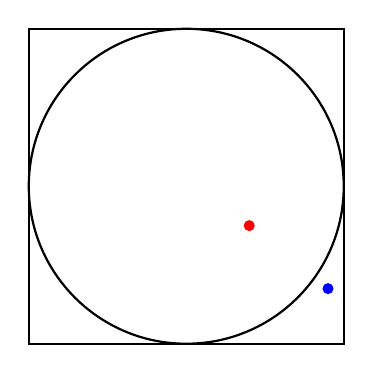
\begin{tikzpicture}
    % Draw the square
    \draw[thick] (0, 0) rectangle (4, 4);

    % Draw the circle
    \draw[thick] (2, 2) circle(2);

    \fill[red] (2.8, 1.5) circle(2pt);
    \fill[blue] (3.8, 0.7) circle(2pt);
    
\end{tikzpicture}
\end{center}
\end{problem}

% 6 Bertrand
\begin{problem}
    Bertrand's paradox
\end{problem}

% 7 Coin flip
\begin{problem}
A fair coin is tossed 3 times. What is the probability of getting at least one tail?
\end{problem}
        
% \begin{problem}
% Two fair dice are rolled. What is the probability of getting $1$ on (at least) one of them, given that their sum is even?
% \end{problem}
% \bigskip

% 8 Urn with balls
\begin{problem}
    An urn contains 3 red balls and 5 blue balls. Two balls are drawn at random without replacement. What is the probability that both balls are red?
\end{problem}

% 9 Deck of cards
\begin{problem}
A standard deck of 52 playing cards is shuffled. What is the probability that the top card is a heart or a queen?
\end{problem}

% \begin{problem}
% There are $15$ books on a bookshelf, $5$ in Armenian, $10$ in French. Ruben cannot read French. If he randomly takes $3$ books, what is the probability that he can read at least one of them?
% \end{problem}



% \bigskip

% \begin{problem}
% $3$ cards are drawn from a deck of $52$ cards. What is the probability that the first two cards are queens, and the third one is diamonds $\blacklozenge$?
% \end{problem}
